% !TEX root = ./jwProj.tex

The aim of this section is to prove the following.

\begin{thm}
\label{thm:main}
The $n$th Jones-Wenzl idempotent is isomorphic to a direct sum of $n+1$ diagrams:

\begin{align*}
p_n &\simeq
\bigoplus_{i=0}^{n}  \iota_{-i} \otimes \iota_{n} \otimes \iota_{-i}\\
&=
\raisebox{2pt}{ \begin{tikzpicture}[mystyle]
    \draw[->](0,0) -- (0,1) node[inner sep=.1cm,below right]{$n$};
    \end{tikzpicture}
}
\oplus \,
\raisebox{2pt}{\begin{tikzpicture}[mystyle] 
    \draw[->](0,1) -- (0,0);
    \draw[->](0.5,0) -- (0.5,1) node[inner sep=0.1cm,below right]{$n$};
    \draw[->](1,1) -- (1,0);
    \end{tikzpicture}
}
\, \oplus \,
\dots
\oplus
\raisebox{2pt}{ \begin{tikzpicture}[mystyle]
    \draw[->](0,1) -- (0,0) node[inner sep=0.1cm,above right]{$n$};
    \draw[->](0.5,0) -- (0.5,1) node[inner sep=0.1cm,below right]{$n$};
    \draw[->](1,1) -- (1,0) node[inner sep=0.1cm,above right]{$n$};
    \end{tikzpicture}
}
\end{align*}
\end{thm}

\begin{proof}
Since $p_n$ is an idempotent, $p_n=p_n^2=p_n \id_n p_n$, where $\id_n$ is $n$ nonoriented parallel strands, the multiplicative identity in $\mathcal{TL}_n^n$.
Now write $\id_n$ as a sum of
$2^n$ different ways of orienting $n$ vertical strands.
Break this sum into $n+1$ sums depending on 
how many strands are oriented up.
 
\begin{defn}
Let $p^k_{n-k}$ denote the sum of $\binom{n}{k}$ diagrams
obtained from $p_n \id_n p_n$
by orienting $k$ strands up and $n-k$ strands down
in the $\id_n$.
\end{defn}
 
Then $p_n = p^0_n + p^1_{n-1} + \dots + p^n_0$.
If $k_1 \neq k_2$, then $p^{k_1}_{n-k_1}p^{k_2}_{n-k_2}=0$.
Thus, by Lemma \ref{lem:dirSum},
$$p_n \simeq p^0_n \oplus p^1_{n-1} \oplus \dots \oplus p^n_0.$$
It remains only to show
$$p^k_l \simeq \iota_{-l} \otimes \iota_{k+l} \otimes \iota_{-l}.$$
This is done in Lemma \ref{lem:isom}.
\end{proof}

To prove Lemma \ref{lem:isom},
we first define $X^k_l$,
which we will show is equal a scalar times $p^k_l$ in Lemma \ref{lem:pkl}.

\begin{defn} \label{defn:x}
%$$X^k_l = \begin{tikzpicture}[mystyle]

\draw [] (-1.4,1) rectangle (1.4,1.2);
\draw [] (-1.4,-1) rectangle (1.4,-1.2);

\begin{scope}[decoration={markings, mark=at position 0.5 with {\arrow{>}}}]
  \draw[postaction={decorate}]
    (1, 1) to[out=270, in=0] node[near start, auto]{$l$} (0.6,0);
  \draw[postaction={decorate}]
    (1, -1) to[out=90, in=0] node[near start, auto, swap]{$k$} (0.6,0);
  \draw[postaction={decorate}]
    (0.6,0) -- (-0.6,0);
  \draw[postaction={decorate}]
    (-0.6,0) to[out=180, in=270] node[near end, auto]{$k$} (-1, 1);
  \draw[postaction={decorate}]
    (-0.6,0) to[out=180, in=90] node[near end, auto, swap]{$l$} (-1, -1);
\end{scope}

\node at (-0.6,0) [inner sep=0.5,above right] {$\scriptstyle{k+l}$};

\draw[->] (0,0.6) +(10:0.2) arc(10:400:0.2) node[right]{$l$};

\draw[->] (0,-0.6) +(400:0.2) arc(400:10:0.2) node[right]{$l$};

\end{tikzpicture}
$$

%$$X^k_l =\begin{tikzpicture}[mystyle]
%\draw [] (-1.4,1) rectangle (1.4,1.2);
%\draw [] (-1.4,-1) rectangle (1.4,-1.2);
%\begin{scope}[decoration={markings, mark=at position 0.5 with {\arrow{>}}}]
%  \draw[postaction={decorate}]
%    (1, 1) to[out=270, in=0] node[near start, auto]{$l$} (0.6,0);
%  \draw[postaction={decorate}]
%    (1, -1) to[out=90, in=0] node[near start, auto, swap]{$k$} (0.6,0);
%  \draw[postaction={decorate}]
%    (0.6,0) -- (-0.6,0);
%  \draw[postaction={decorate}]
%    (-0.6,0) to[out=180, in=270] node[near end, auto]{$k$} (-1, 1);
%  \draw[postaction={decorate}]
%    (-0.6,0) to[out=180, in=90] node[near end, auto, swap]{$l$} (-1, -1);
%\end{scope}
%\node at (-0.6,0) [inner sep=0.5,above right] {$\scriptstyle{k+l}$};
%\draw[->] (0,0.6) +(10:0.2) arc(10:400:0.2) node[right]{$l$};
%\draw[->] (0,-0.6) +(400:0.2) arc(400:10:0.2) node[right]{$l$};
%\end{tikzpicture}$$

$$X^k_l = \vcenter{\hbox{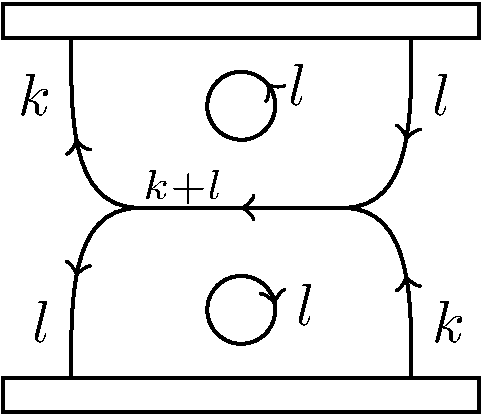
\includegraphics[scale=.275]{mainThm/diagrams/xkl_.pdf}}}$$
%= \vcenter{\hbox{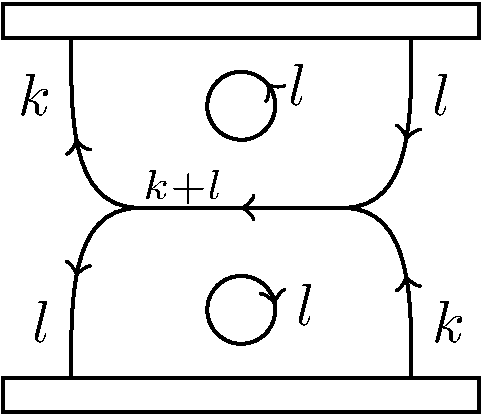
\includegraphics[scale=.275, clip]{mainThm/diagrams/xkl_.pdf}}}
%=\begin{tikzpicture}[mystyle]

\draw [] (-1.4,1) rectangle (1.4,1.2);
\draw [] (-1.4,-1) rectangle (1.4,-1.2);

\begin{scope}[decoration={markings, mark=at position 0.5 with {\arrow{>}}}]
  \draw[postaction={decorate}]
    (1, 1) to[out=270, in=0] node[near start, auto]{$l$} (0.6,0);
  \draw[postaction={decorate}]
    (1, -1) to[out=90, in=0] node[near start, auto, swap]{$k$} (0.6,0);
  \draw[postaction={decorate}]
    (0.6,0) -- (-0.6,0);
  \draw[postaction={decorate}]
    (-0.6,0) to[out=180, in=270] node[near end, auto]{$k$} (-1, 1);
  \draw[postaction={decorate}]
    (-0.6,0) to[out=180, in=90] node[near end, auto, swap]{$l$} (-1, -1);
\end{scope}

\node at (-0.6,0) [inner sep=0.5,above right] {$\scriptstyle{k+l}$};

\draw[->] (0,0.6) +(10:0.2) arc(10:400:0.2) node[right]{$l$};

\draw[->] (0,-0.6) +(400:0.2) arc(400:10:0.2) node[right]{$l$};

\end{tikzpicture}
$$
\end{defn}

Lemmas \ref{lem:xkm1l} and \ref{lem:xklm1} are similar and begin the inductive step of the proof of Lemma \ref{lem:pkl}.

\begin{lem}\label{lem:xkm1l}
$p_{k+l} (X^{k-1}_l \otimes \iota_1) p_{k+l} = (-1)^{l} X^k_l \otimes \beta_{-l}.$
\end{lem}

\begin{proof}
 \begin{align*}
 p_{k+l} (X^{k-1}_l \otimes \iota_1) p_{k+l} &= \vcenter{\hbox{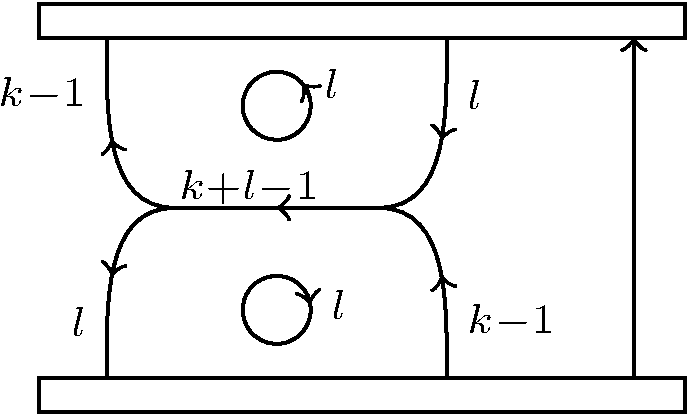
\includegraphics[scale=.275]{mainThm/diagrams/xkm1l_a_.pdf}}}\\%\begin{tikzpicture}[mystyle]

\draw [] (-1.4,1) rectangle (2.4,1.2);
\draw [] (-1.4,-1) rectangle (2.4,-1.2);

\begin{scope}[decoration={markings, mark=at position 0.5 with {\arrow{>}}}]
  \draw[postaction={decorate}]
    (1, 1) to[out=270, in=0] node[near start, auto]{$\scriptstyle{l}$} (0.6,0);
  \draw[postaction={decorate}]
    (1, -1) to[out=90, in=0] node[near start, auto, swap]{$\scriptstyle{k-1}$} (0.6,0);
  \draw[postaction={decorate}]
    (0.6,0) -- (-0.6,0);
  \draw[postaction={decorate}]
    (-0.6,0) to[out=180, in=270] node[near end, auto]{$\scriptstyle{k-1}$} (-1, 1);
  \draw[postaction={decorate}]
    (-0.6,0) to[out=180, in=90] node[near end, auto, swap]{$\scriptstyle{l}$} (-1, -1);
\end{scope}

\node at (-0.6,0) [inner sep=0.5,above right] {$\scriptstyle{k+l-1}$};

%\draw[ 
%        decoration={markings, mark=at position 0.7 with {\arrow{<}}},
%        postaction={decorate}
%]
%       (1.4,-1.2) -- (-1.4, 1.2);
\draw[->] (2.1,-1) --(2.1,1) ;



\draw[->] (0,0.6) +(10:0.2) arc(10:400:0.2) node[right]{$\scriptstyle{l}$};

\draw[->] (0,-0.6) +(400:0.2) arc(400:10:0.2) node[right]{$\scriptstyle{l}$};

\end{tikzpicture}
\\
 \intertext{By a pop-switch relation we have the following.}\\
 &= \vcenter{\hbox{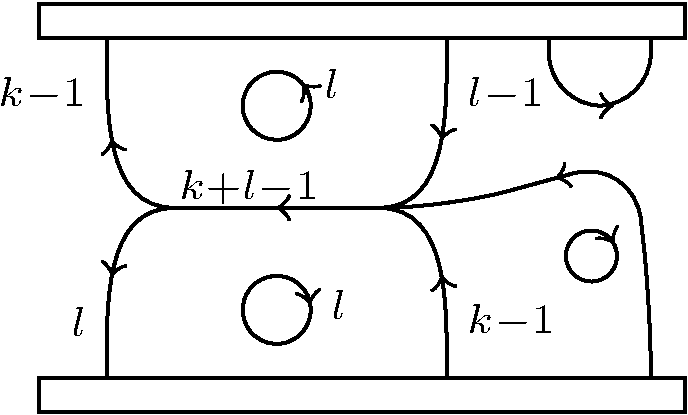
\includegraphics[scale=.275]{mainThm/diagrams/xkm1l_b_.pdf}}}\\%\begin{tikzpicture}[mystyle]

\draw [] (-1.4,1) rectangle (2.4,1.2);
\draw [] (-1.4,-1) rectangle (2.4,-1.2);

\begin{scope}[decoration={markings, mark=at position 0.5 with {\arrow{>}}}]
  \draw[postaction={decorate}]
    (1, 1) to[out=270, in=0] node[near start, auto]{$\scriptstyle{l-1}$} (0.6,0);
  \draw[postaction={decorate}]
    (1, -1) to[out=90, in=0] node[near start, auto, swap]{$\scriptstyle{k-1}$} (0.6,0);
  \draw[postaction={decorate}]
    (0.6,0) -- (-0.6,0);
  \draw[postaction={decorate}]
    (-0.6,0) to[out=180, in=270] node[near end, auto]{$\scriptstyle{k-1}$} (-1, 1);
  \draw[postaction={decorate}]
    (-0.6,0) to[out=180, in=90] node[near end, auto, swap]{$\scriptstyle{l}$} (-1, -1);
\end{scope}

\node at (-0.6,0) [inner sep=0.5,above right] {$\scriptstyle{k+l-1}$};

\draw[->] (0,0.6) +(10:0.2) arc(10:400:0.2) node[right]{$\scriptstyle{l}$};

\draw[->] (0,-0.6) +(400:0.2) arc(400:10:0.2) node[right]{$\scriptstyle{l}$};


\arc{1}{.4}{1.9}{}{<}
\draw[->] (1.8,-0.2) +(400:0.1) arc(440:30:0.15);

\draw[rounded corners=.3cm,
        decoration={markings, mark=at position 0.6 with {\arrow{>}}},
        postaction={decorate}]
   (2.2,-1) --(2.2,-.6) --(2.1,0.3)--(1,0)--(.6,0) ;


\end{tikzpicture}
\\
 \intertext{Then by Lemma \ref{lem:arcMove} we can move the arc across the $l-1$ strands creating a $\beta_{l-1}$ on the right.  Next we use Lemma \ref{lem:oio} to replace the arc with $\beta_{-1}\otimes\iota_{1}\otimes\beta_{1}$.}\\
 &=(-1)^l \vcenter{\hbox{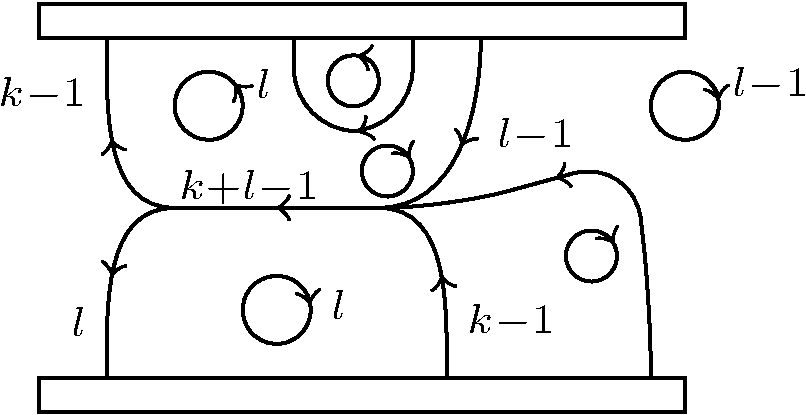
\includegraphics[scale=.275]{mainThm/diagrams/xkm1l_d_.pdf}}}\\%\begin{tikzpicture}[mystyle]

\draw [] (-1.4,1) rectangle (2.4,1.2);
\draw [] (-1.4,-1) rectangle (2.4,-1.2);

\begin{scope}[decoration={markings, mark=at position 0.5 with {\arrow{>}}}]
  \draw[postaction={decorate}]
    (1.2, 1) to[out=270, in=0] node[near start, auto]{$\scriptstyle{l-1}$} (0.6,0);
  \draw[postaction={decorate}]
    (1, -1) to[out=90, in=0] node[near start, auto, swap]{$\scriptstyle{k-1}$} (0.6,0);
  \draw[postaction={decorate}]
    (0.6,0) -- (-0.6,0);
  \draw[postaction={decorate}]
    (-0.6,0) to[out=180, in=270] node[near end, auto]{$\scriptstyle{k-1}$} (-1, 1);
  \draw[postaction={decorate}]
    (-0.6,0) to[out=180, in=90] node[near end, auto, swap]{$\scriptstyle{l}$} (-1, -1);

%\draw[postaction={decorate}] (2.2,-1) to[out=90, in=180] (0.6, 0);
% -- ++(90:.5cm) arc(0:115:.5)arc(295:180:.5) --++(0.6,0);
\end{scope}

\node at (-0.6,0) [inner sep=0.5,above right] {$\scriptstyle{k+l-1}$};

\draw[->] (-0.4,0.6) +(10:0.2) arc(10:400:0.2) node[right]{$\scriptstyle{l}$};

\draw[->] (0,-0.6) +(400:0.2) arc(400:10:0.2) node[right]{$\scriptstyle{l}$};

\draw[<-] (2.4,0.6) +(10:0.2) arc(10:400:0.2) node[right]{$\scriptstyle{l-1}$};


%\arc{1}{.4}{0.4}{}{>}
\draw[rounded corners=.3cm,
        decoration={markings, mark=at position 0.6 with {\arrow{<}}},
        postaction={decorate}]
   (0.1,1) --(0.1,.45) --(0.8,.45)--(.8,1) ;

\draw[<-] (0.4,0.83) +(400:0.1) arc(440:50:0.15);
\draw[->] (0.6,0.3) +(400:0.1) arc(440:30:0.15);

\draw[->] (1.8,-0.2) +(400:0.1) arc(440:30:0.15); 



\draw[rounded corners=.3cm,
        decoration={markings, mark=at position 0.6 with {\arrow{>}}},
        postaction={decorate}]
   (2.2,-1) --(2.2,-.6) --(2.1,0.3)--(1,0)--(.6,0) ;


\end{tikzpicture}
\\
 \intertext{Move the innermost $\beta_1$ from the $\beta_l$ to the far right across $l-1$ strands in both directions by Lemma \ref{lem:teleport}.}\\
 &=(-1)^l \vcenter{\hbox{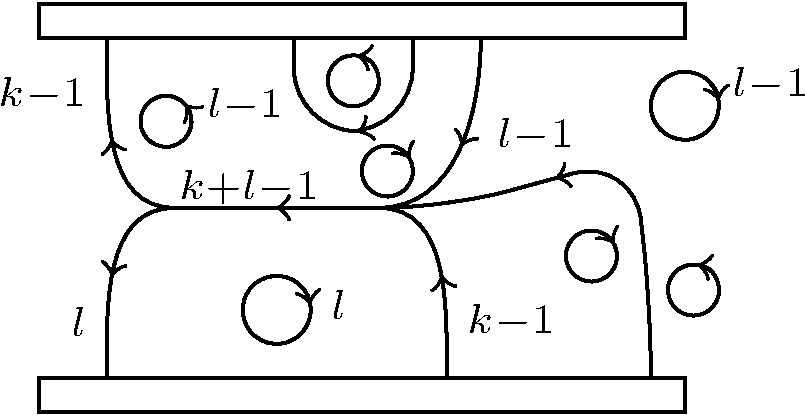
\includegraphics[scale=.275]{mainThm/diagrams/xkm1l_e_.pdf}}}\\%\begin{tikzpicture}[mystyle]

\draw [] (-1.4,1) rectangle (2.4,1.2);
\draw [] (-1.4,-1) rectangle (2.4,-1.2);

\begin{scope}[decoration={markings, mark=at position 0.5 with {\arrow{>}}}]
  \draw[postaction={decorate}]
    (1.2, 1) to[out=270, in=0] node[near start, auto]{$\scriptstyle{l-1}$} (0.6,0);
  \draw[postaction={decorate}]
    (1, -1) to[out=90, in=0] node[near start, auto, swap]{$\scriptstyle{k-1}$} (0.6,0);
  \draw[postaction={decorate}]
    (0.6,0) -- (-0.6,0);
  \draw[postaction={decorate}]
    (-0.6,0) to[out=180, in=270] node[near end, auto]{$\scriptstyle{k-1}$} (-1, 1);
  \draw[postaction={decorate}]
    (-0.6,0) to[out=180, in=90] node[near end, auto, swap]{$\scriptstyle{l}$} (-1, -1);

%\draw[postaction={decorate}] (2.2,-1) to[out=90, in=180] (0.6, 0);
% -- ++(90:.5cm) arc(0:115:.5)arc(295:180:.5) --++(0.6,0);
\end{scope}

\node at (-0.6,0) [inner sep=0.5,above right] {$\scriptstyle{k+l-1}$};

\draw[->] (-0.7,0.5) +(10:0.2) arc(10:400:0.15) node[right]{$\scriptstyle{l-1}$};

\draw[->] (0,-0.6) +(400:0.2) arc(400:10:0.2) node[right]{$\scriptstyle{l}$};

\draw[<-] (2.4,0.6) +(10:0.2) arc(10:400:0.2) node[right]{$\scriptstyle{l-1}$};


%\arc{1}{.4}{0.4}{}{>}
\draw[rounded corners=.3cm,
        decoration={markings, mark=at position 0.6 with {\arrow{<}}},
        postaction={decorate}]
   (0.1,1) --(0.1,.45) --(0.8,.45)--(.8,1) ;

\draw[<-] (0.4,0.83) +(400:0.1) arc(440:50:0.15);
\draw[->] (0.6,0.3) +(400:0.1) arc(440:30:0.15);

\draw[<-] (2.4,-0.4) +(400:0.1) arc(440:50:0.15);
\draw[->] (1.8,-0.2) +(400:0.1) arc(440:30:0.15);

%\draw[<-] (1.8,-0.2) +(10:0.2) arc(10:400:0.15); 
%\draw[->] (2.4,-0.4) +(10:0.2) arc(10:400:0.15); 



\draw[rounded corners=.3cm,
        decoration={markings, mark=at position 0.6 with {\arrow{>}}},
        postaction={decorate}]
   (2.2,-1) --(2.2,-.6) --(2.1,0.3)--(1,0)--(.6,0) ;


\end{tikzpicture}
\\
  \intertext{Then remove the two bubbles on the bottom right of the diagram by Lemma \ref{lem:oio}.}\\
 &=(-1)^l\vcenter{\hbox{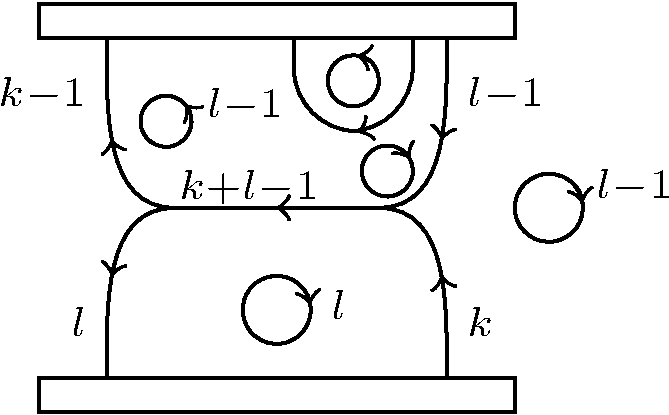
\includegraphics[scale=.275]{mainThm/diagrams/xkm1l_f_.pdf}}}\\%\begin{tikzpicture}[mystyle]

\draw [] (-1.4,1) rectangle (1.4,1.2);
\draw [] (-1.4,-1) rectangle (1.4,-1.2);

\begin{scope}[decoration={markings, mark=at position 0.5 with {\arrow{>}}}]
  \draw[postaction={decorate}]
    (1, 1) to[out=270, in=0] node[near start, auto]{$\scriptstyle{l-1}$} (0.6,0);
  \draw[postaction={decorate}]
    (1, -1) to[out=90, in=0] node[near start, auto, swap]{$\scriptstyle{k}$} (0.6,0);
  \draw[postaction={decorate}]
    (0.6,0) -- (-0.6,0);
  \draw[postaction={decorate}]
    (-0.6,0) to[out=180, in=270] node[near end, auto]{$\scriptstyle{k-1}$} (-1, 1);
  \draw[postaction={decorate}]
    (-0.6,0) to[out=180, in=90] node[near end, auto, swap]{$\scriptstyle{l}$} (-1, -1);
\end{scope}

\node at (-0.6,0) [inner sep=0.5,above right] {$\scriptstyle{k+l-1}$};

\draw[->] (-0.7,0.5) +(10:0.2) arc(10:400:0.15) node[right]{$\scriptstyle{l-1}$};

\draw[->] (0,-0.6) +(400:0.2) arc(400:10:0.2) node[right]{$\scriptstyle{l}$};

\draw[<-] (1.6,0.0) +(10:0.2) arc(10:400:0.2) node[right]{$\scriptstyle{l-1}$};

\draw[rounded corners=.3cm,
        decoration={markings, mark=at position 0.6 with {\arrow{<}}},
        postaction={decorate}]
   (0.1,1) --(0.1,.45) --(0.8,.45)--(.8,1) ;


\draw[<-] (0.4,0.83) +(400:0.1) arc(440:50:0.15);
\draw[->] (0.6,0.3) +(400:0.1) arc(440:30:0.15);


\end{tikzpicture}
\\
   \intertext{Lastly, by Lemma \ref{lem:teleport} move the $\beta_{l-1}$ into the $\beta_{1}$ and the $\beta_{-1}$ into the $\beta_{-(l-1)}$.}\\
 &=(-1)^l \vcenter{\hbox{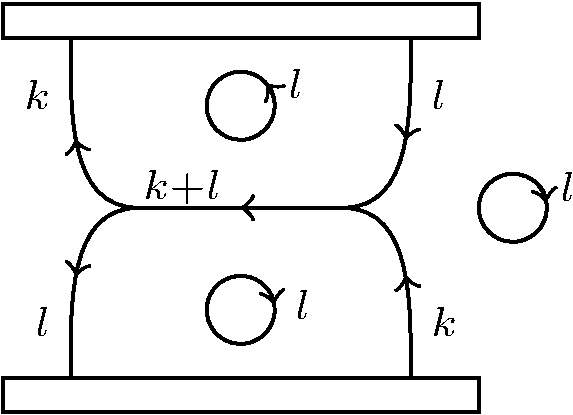
\includegraphics[scale=.275]{mainThm/diagrams/xkm1l_g_.pdf}}}\\[.3cm]%\begin{tikzpicture}[mystyle]

\draw [] (-1.4,1) rectangle (1.4,1.2);
\draw [] (-1.4,-1) rectangle (1.4,-1.2);

\begin{scope}[decoration={markings, mark=at position 0.5 with {\arrow{>}}}]
  \draw[postaction={decorate}]
    (1, 1) to[out=270, in=0] node[near start, auto]{$\scriptstyle{l}$} (0.6,0);
  \draw[postaction={decorate}]
    (1, -1) to[out=90, in=0] node[near start, auto, swap]{$\scriptstyle{k}$} (0.6,0);
  \draw[postaction={decorate}]
    (0.6,0) -- (-0.6,0);
  \draw[postaction={decorate}]
    (-0.6,0) to[out=180, in=270] node[near end, auto]{$\scriptstyle{k}$} (-1, 1);
  \draw[postaction={decorate}]
    (-0.6,0) to[out=180, in=90] node[near end, auto, swap]{$\scriptstyle{l}$} (-1, -1);
\end{scope}

\node at (-0.6,0) [inner sep=0.5,above right] {$\scriptstyle{k+l}$};


\draw[->] (0,0.6) +(10:0.2) arc(10:400:0.2) node[right]{$\scriptstyle{l}$};

\draw[->] (0,-0.6) +(400:0.2) arc(400:10:0.2) node[right]{$\scriptstyle{l}$};


\draw[<-] (1.6,0.0) +(10:0.2) arc(10:400:0.2) node[right]{$\scriptstyle{l}$};





\end{tikzpicture}
\\[.3cm]
 &=(-1)^{l} X^k_l \otimes \beta_{-l}\\
 \end{align*}
\end{proof}

\begin{lem}\label{lem:xklm1}
$p_{k+l} (X^k_{l-1} \otimes \iota_{-1}) p_{k+l} =
  (-1)^{k} X^k_l \otimes \beta_k.$
\end{lem}

\begin{proof}
 \begin{align*}
 p_{k+l} (X^{k}_{l-1} \otimes \iota_{-1}) p_{k+l} &=\vcenter{\hbox{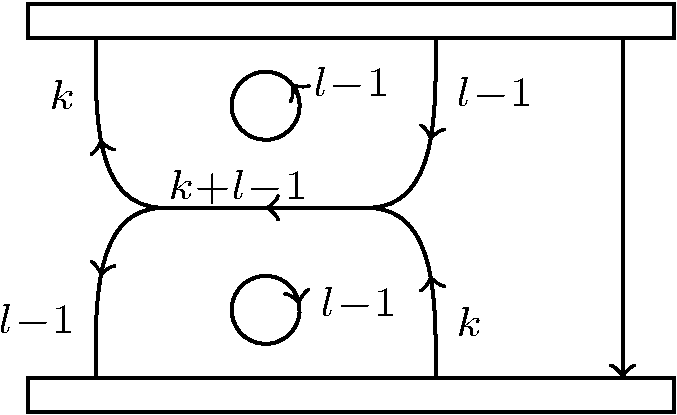
\includegraphics[scale=.275]{mainThm/diagrams/xklm1_a_.pdf}}}\\%\begin{tikzpicture}[mystyle]

\draw [] (-1.4,1) rectangle (2.4,1.2);
\draw [] (-1.4,-1) rectangle (2.4,-1.2);

\begin{scope}[decoration={markings, mark=at position 0.5 with {\arrow{>}}}]
  \draw[postaction={decorate}]
    (1, 1) to[out=270, in=0] node[near start, auto]{$\scriptstyle{l-1}$} (0.6,0);
  \draw[postaction={decorate}]
    (1, -1) to[out=90, in=0] node[near start, auto, swap]{$\scriptstyle{k}$} (0.6,0);
  \draw[postaction={decorate}]
    (0.6,0) -- (-0.6,0);
  \draw[postaction={decorate}]
    (-0.6,0) to[out=180, in=270] node[near end, auto]{$\scriptstyle{k}$} (-1, 1);
  \draw[postaction={decorate}]
    (-0.6,0) to[out=180, in=90] node[near end, auto, swap]{$\scriptstyle{l-1}$} (-1, -1);
\end{scope}

\node at (-0.6,0) [inner sep=0.5,above right] {$\scriptstyle{k+l-1}$};

%\draw[ 
%        decoration={markings, mark=at position 0.7 with {\arrow{<}}},
%        postaction={decorate}
%]
%       (1.4,-1.2) -- (-1.4, 1.2);
\draw[<-] (2.1,-1) --(2.1,1) ;



\draw[->] (0,0.6) +(10:0.2) arc(10:400:0.2) node[right]{$\scriptstyle{l-1}$};

\draw[->] (0,-0.6) +(400:0.2) arc(400:10:0.2) node[right]{$\scriptstyle{l-1}$};

\end{tikzpicture}
\\
 \intertext{By a pop-switch relation we have the following.}\\
 &=\vcenter{\hbox{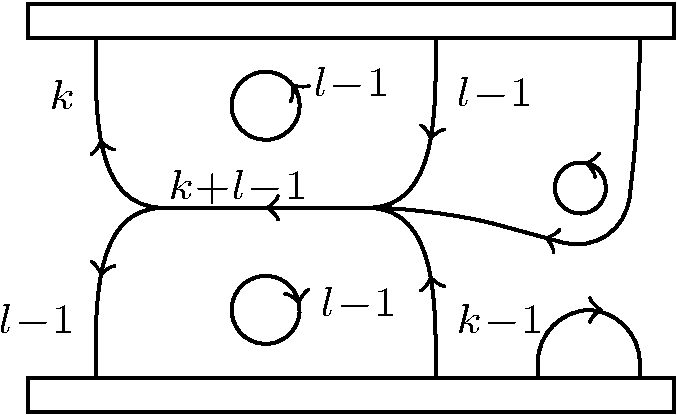
\includegraphics[scale=.275]{mainThm/diagrams/xklm1_b_.pdf}}}\\%\begin{tikzpicture}[mystyle]

\draw [] (-1.4,1) rectangle (2.4,1.2);
\draw [] (-1.4,-1) rectangle (2.4,-1.2);

\begin{scope}[decoration={markings, mark=at position 0.5 with {\arrow{>}}}]
  \draw[postaction={decorate}]
    (1, 1) to[out=270, in=0] node[near start, auto]{$\scriptstyle{l-1}$} (0.6,0);
  \draw[postaction={decorate}]
    (1, -1) to[out=90, in=0] node[near start, auto, swap]{$\scriptstyle{k-1}$} (0.6,0);
  \draw[postaction={decorate}]
    (0.6,0) -- (-0.6,0);
  \draw[postaction={decorate}]
    (-0.6,0) to[out=180, in=270] node[near end, auto]{$\scriptstyle{k}$} (-1, 1);
  \draw[postaction={decorate}]
    (-0.6,0) to[out=180, in=90] node[near end, auto, swap]{$\scriptstyle{l-1}$} (-1, -1);
\end{scope}

\node at (-0.6,0) [inner sep=0.5,above right] {$\scriptstyle{k+l-1}$};

\arc{-1}{-.4}{1.9}{}{<}

\draw[<-] (1.8,0.2) +(400:0.1) arc(440:30:0.15);

\draw[rounded corners=.3cm,
        decoration={markings, mark=at position 0.6 with {\arrow{>}}},
        postaction={decorate}]
   (2.2,1) --(2.2,.6) --(2.1,-0.3)--(1,0)--(.6,0) ;


\draw[->] (0,0.6) +(10:0.2) arc(10:400:0.2) node[right]{$\scriptstyle{l-1}$};

\draw[->] (0,-0.6) +(400:0.2) arc(400:10:0.2) node[right]{$\scriptstyle{l-1}$};

\end{tikzpicture}
\\
 \intertext{Then by Lemma \ref{lem:arcMove} we can move the arc across the $k-1$ strands creating a $\beta_{-(k-1)}$ on the right.  Next we use Lemma \ref{lem:teleport} to move the $\beta_1$ across the $l-1$ strands in both directions into the $\beta_{l-1}$.}\\
 &=(-1)^k \vcenter{\hbox{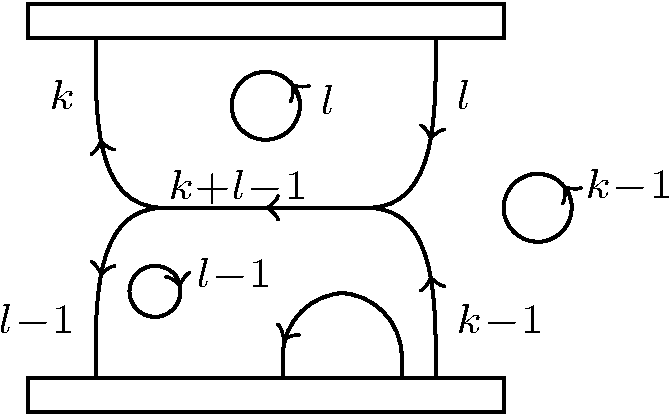
\includegraphics[scale=.275]{mainThm/diagrams/xklm1_c_.pdf}}}\\%%%xklm1_c
\begin{tikzpicture}[mystyle]

\draw [] (-1.4,1) rectangle (1.4,1.2);
\draw [] (-1.4,-1) rectangle (1.4,-1.2);

\begin{scope}[decoration={markings, mark=at position 0.5 with {\arrow{>}}}]
  \draw[postaction={decorate}]
    (1, 1) to[out=270, in=0] node[near start, auto]{$\scriptstyle{l}$} (0.6,0);
  \draw[postaction={decorate}]
    (1, -1) to[out=90, in=0] node[near start, auto, swap]{$\scriptstyle{k-1}$} (0.6,0);
  \draw[postaction={decorate}]
    (0.6,0) -- (-0.6,0);
  \draw[postaction={decorate}]
    (-0.6,0) to[out=180, in=270] node[near end, auto]{$\scriptstyle{k}$} (-1, 1);
  \draw[postaction={decorate}]
    (-0.6,0) to[out=180, in=90] node[near end, auto, swap]{$\scriptstyle{l-1}$} (-1, -1);
\end{scope}

\node at (-0.6,0) [inner sep=0.5,above right] {$\scriptstyle{k+l-1}$};

\draw[<-] (-0.7,-0.5) +(10:0.2) arc(10:400:0.15) node[right]{$\scriptstyle{l-1}$};

\draw[<-] (0,0.6) +(400:0.2) arc(400:10:0.2) node[right]{$\scriptstyle{l}$};

\draw[->] (1.6,0.0) +(10:0.2) arc(10:400:0.2) node[right]{$\scriptstyle{k-1}$};

\draw[rounded corners=.3cm,
        decoration={markings, mark=at position 0.2 with {\arrow{<}}},
        postaction={decorate}]
   (0.1,-1) --(0.1,-.5) --(0.8,-.5)--(.8,-1) ;



%\draw[->] (0.4,-0.72) +(400:0.1) arc(440:50:0.15);
%\draw[<-] (0.6,-0.2) +(400:0.1) arc(440:30:0.15);


\end{tikzpicture}
\\
 \intertext{Replace the arc with $\beta_{-1}\otimes\iota_{1}\otimes\beta_{1}$.}\\
 &=(-1)^k \vcenter{\hbox{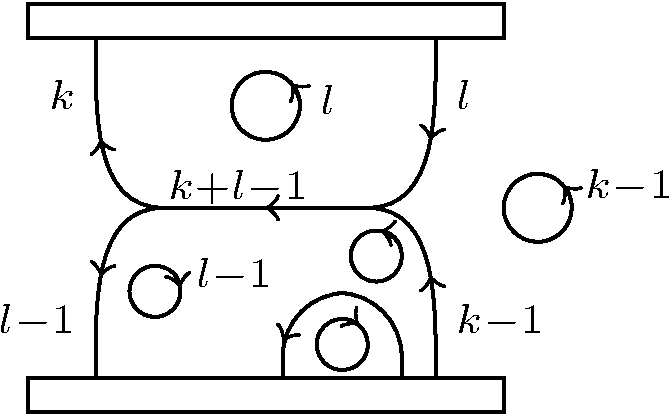
\includegraphics[scale=.275]{mainThm/diagrams/xklm1_d_.pdf}}}\\%\begin{tikzpicture}[mystyle]

\draw [] (-1.4,1) rectangle (1.4,1.2);
\draw [] (-1.4,-1) rectangle (1.4,-1.2);

\begin{scope}[decoration={markings, mark=at position 0.5 with {\arrow{>}}}]
  \draw[postaction={decorate}]
    (1, 1) to[out=270, in=0] node[near start, auto]{$\scriptstyle{l}$} (0.6,0);
  \draw[postaction={decorate}]
    (1, -1) to[out=90, in=0] node[near start, auto, swap]{$\scriptstyle{k-1}$} (0.6,0);
  \draw[postaction={decorate}]
    (0.6,0) -- (-0.6,0);
  \draw[postaction={decorate}]
    (-0.6,0) to[out=180, in=270] node[near end, auto]{$\scriptstyle{k}$} (-1, 1);
  \draw[postaction={decorate}]
    (-0.6,0) to[out=180, in=90] node[near end, auto, swap]{$\scriptstyle{l-1}$} (-1, -1);
\end{scope}

\node at (-0.6,0) [inner sep=0.5,above right] {$\scriptstyle{k+l-1}$};

\draw[<-] (-0.7,-0.5) +(10:0.2) arc(10:400:0.15) node[right]{$\scriptstyle{l-1}$};

\draw[<-] (0,0.6) +(400:0.2) arc(400:10:0.2) node[right]{$\scriptstyle{l}$};

\draw[->] (1.6,0.0) +(10:0.2) arc(10:400:0.2) node[right]{$\scriptstyle{k-1}$};

\draw[rounded corners=.3cm,
        decoration={markings, mark=at position 0.2 with {\arrow{<}}},
        postaction={decorate}]
   (0.1,-1) --(0.1,-.5) --(0.8,-.5)--(.8,-1) ;



\draw[->] (0.4,-0.72) +(400:0.1) arc(440:50:0.15);
\draw[<-] (0.6,-0.2) +(400:0.1) arc(440:30:0.15);


\end{tikzpicture}
\\
   \intertext{Lastly, by Lemma \ref{lem:teleport} move the $\beta_1$ across the $k-1$ strands in both directions into the $\beta_{k-1}$.  By the same lemma, move the $\beta_{-(l-1)}$ into the $\beta_{-1}$.}\\
 &=(-1)^k \vcenter{\hbox{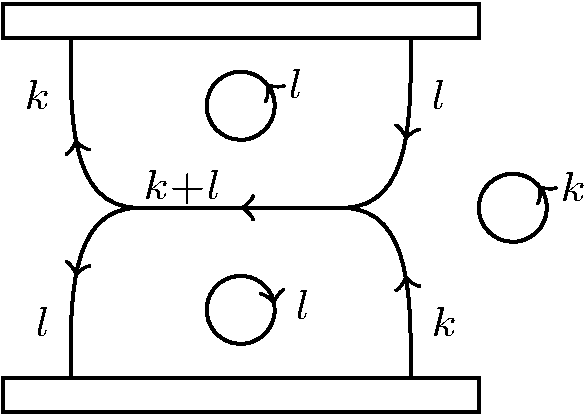
\includegraphics[scale=.275]{mainThm/diagrams/xklm1_e_.pdf}}}\\%\begin{tikzpicture}[mystyle]

\draw [] (-1.4,1) rectangle (1.4,1.2);
\draw [] (-1.4,-1) rectangle (1.4,-1.2);

\begin{scope}[decoration={markings, mark=at position 0.5 with {\arrow{>}}}]
  \draw[postaction={decorate}]
    (1, 1) to[out=270, in=0] node[near start, auto]{$\scriptstyle{l}$} (0.6,0);
  \draw[postaction={decorate}]
    (1, -1) to[out=90, in=0] node[near start, auto, swap]{$\scriptstyle{k}$} (0.6,0);
  \draw[postaction={decorate}]
    (0.6,0) -- (-0.6,0);
  \draw[postaction={decorate}]
    (-0.6,0) to[out=180, in=270] node[near end, auto]{$\scriptstyle{k}$} (-1, 1);
  \draw[postaction={decorate}]
    (-0.6,0) to[out=180, in=90] node[near end, auto, swap]{$\scriptstyle{l}$} (-1, -1);
\end{scope}

\node at (-0.6,0) [inner sep=0.5,above right] {$\scriptstyle{k+l}$};


\draw[->] (0,0.6) +(10:0.2) arc(10:400:0.2) node[right]{$\scriptstyle{l}$};

\draw[->] (0,-0.6) +(400:0.2) arc(400:10:0.2) node[right]{$\scriptstyle{l}$};


\draw[->] (1.6,0.0) +(10:0.2) arc(10:400:0.2) node[right]{$\scriptstyle{k}$};





\end{tikzpicture}
\\[.3cm]
 &=(-1)^{k} X^k_l \otimes \beta_{k}\\
 \end{align*}
\end{proof}

Lemma \ref{lem:bubbs} is the key to proving Lemma \ref{lem:quantPT}, which is required to complete the proof of Lemma \ref{lem:pkl}.
  It is worth noting that  in Lemma \ref{lem:quantPT} the $X^k_l$ merely acts as a catalyst to provide enough strands to use \ref{lem:bubbs}. 
All that is necessary is the presence of $\iota_{-l+1}$ and $\iota_{k-1}$ on the left as specified in Lemma \ref{lem:bubbs} for the purpose of implementing Corollary \ref{cor:ia}.  

\begin{lem}\label{lem:bubbs}
For $k\geq n-1$,
$$\iota_k\otimes \beta_n = [n]\iota_k\otimes\beta_1-[n-1]\iota_k$$
and
$$\iota_{-k}\otimes \beta_{-n} = [n]\iota_{-k}\otimes\beta_{-1}-[n-1]\iota_{-k}$$
\end{lem}

\begin{proof}
We prove the first identity, since the second is similar.
Consider the case $n=2$ with $k\geq 1$.
Use the bubble-bursting relation on the innermost loop of $\beta_2$.
Corollary \ref{cor:ia} then gives the result.
$$\iota_k\otimes \beta_2 = [2] \iota_k\otimes \beta_1 - \iota_k\otimes \alpha_1 = [2] \iota_k\otimes \beta_1 - \iota_k$$

Now assume $k\geq n-1$.
Use the bubble-bursting relation on the innermost loop of $\beta_n$.
Corollary \ref{cor:ab}, Corollary \ref{cor:ia}, and induction give
\begin{align*}
\iota_k\otimes \beta_n &= [2] \iota_k\otimes \beta_{n-1} - \iota_k\otimes \beta_{n-2} \\
&=[2]([n-1]\iota_k\otimes\beta_1 - [n-2] \iota_k)-([n-2]\iota_k\otimes\beta_1-[n-3]\iota_k)\\
&=([2][n-1]-[n-2])\iota_k\otimes \beta_1-([2][n-]-[n-3])\iota_k\\
&=[n]\iota_k\otimes\beta_1-[n-1]\iota_k
\end{align*}
\end{proof}

%The following lemma is designed for the induction in the proof of Lemma \ref{lem:pkl}.
%It is worth noting that the $X^k_l$ merely acts as a catalyst to use Corollary \ref{cor:ia}.
%All that is necessary is the presence of $\iota_{-l+1}$ and $\iota_{k-1}$ on the left.

\begin{lem}\label{lem:quantPT}
If $k + l = n$ then
$$ \qbinom{n-1}{l}X^k_l\otimes\beta_{-l} + \qbinom{n-1}{k} X^k_l\otimes\beta_k = \qbinom{n}{k}X^k_l.$$
\end{lem}

\begin{proof}
Note that every term in the equation contains $X^k_l$.
However, the result will hold so long as there are both a $\iota_{-l+1}$ and $\iota_{k-1}$ on the left of each diagram in order to use Lemma \ref{lem:bubbs}.
Thus it suffices to prove
$$ \qbinom{n-1}{l}([l] \beta_{-1} - [l-1]) + \qbinom{n-1}{k}([k] \beta_1 - [k-1]) = \qbinom{n}{k}. $$
Use the identity
$$\qbinom{n-1}{l} [l] = \qbinom{n-1}{k} [k],$$
and the bubble bursting relation $\beta_{-1} + \beta_1 = [2]$
to eliminate $\beta_{-1}$ and $\beta_1$ from the left side.
Then simplify further using the identity $[2][l] - [l-1] = [l+1]$.
We obtain
$$\qbinom{n-1}{l}[l+1] - \qbinom{n-1}{k}[k-1].$$
By Corollary \ref{cor:q},
this is equal to $\qbinom{n}{k}$, as desired.
\end{proof}

\begin{lem} \label{lem:pkl}
$p^k_l = (-1)^{kl} \qbinom{k+l}{k} X^k_l$
\end{lem}

\begin{proof}
Induct on $n=k+l$.  Notice $p^1_0=\iota_1=X^1_0$ and $p^0_1=\iota_{-1}=X^0_1$.  Assume $k>0$ and $l>0$. Then 

\begin{align*}
p^k_l&=p_{k+l}(p^{k-1}_l\otimes\iota_1)p_{k+l}+p_{k+l}(p^{k}_{l-1}\otimes\iota_{-1})p_{k+l}
\intertext{By Lemma \ref{lem:xkm1l} and Lemma \ref{lem:xklm1},}
&=(-1)^{kl}\qbinom{k+l-1}{l}X^k_l\otimes\beta_{-l}+(-1)^{kl}\qbinom{k+l-1}{k}X^k_l\otimes\beta_{k}
\intertext{By Lemma \ref{lem:quantPT},}
&=(-1)^{kl}\qbinom{k+l}{k}X^k_l
\end{align*}

\end{proof}

\begin{lem}\label{lem:isom}
$p^k_l \simeq \iota_{-l} \otimes \iota_{k+l} \otimes \iota_{-l}$.
\end{lem}
\begin{proof}
The explicit isomorphisms are:
$$
f= (-1)^{kl}\qbinom{k+l}{k} \begin{tikzpicture}[mystyle]

\draw [] (-1.4,0.1) rectangle (1.4,-0.1);

% \begin{scope}[decoration={markings, mark=at position 0.5 with {\arrow{>}}}]
%   \draw[postaction={decorate}]
%     (1, 0.1) to[out=90, in=-90] node[near start, auto, swap]{$\scriptstyle{k}$} (0.6,1.1);
%   \draw[postaction={decorate}]
%     (-0.6,1.1) to[out=-90, in=90] node[near end, auto, swap]{$\scriptstyle{l}$} (-1, 0.1);
% \end{scope}

% \draw[->] (0,0.5) +(400:0.2) arc(400:10:0.2) node[right]{$\scriptstyle{l}$};

% \draw[->] (2,1.1)  arc(0:-90:0.3) node[below]{$\scriptstyle{l}$};
% \draw[] (2,1.1)  arc(0:-180:0.3);

\begin{scope}[decoration={markings, mark=at position 0.5 with {\arrow{>}}}]
 \draw[postaction={decorate}]
    (1, -.1) to[out=270, in=90] node[near start, auto]{$\scriptstyle{l}$} (0.6,-1.1);
 \draw[postaction={decorate}]
    (-0.6,-1.1) to[out=90, in=270] node[near end, auto]{$\scriptstyle{k}$} (-1, -.1);
\end{scope}

\draw[<-] (0,-0.5) +(400:0.2) arc(400:10:0.2) node[right]{$\scriptstyle{l}$};

\draw[->] (-1.4,-1.1)  arc(0:90:0.3) node[above]{$\scriptstyle{l}$};
\draw[] (-1.4,-1.1)  arc(0:180:0.3);


\end{tikzpicture}
,
\qquad
g=  \begin{tikzpicture}[mystyle]

\draw [] (-1.4,0.1) rectangle (1.4,-0.1);

\begin{scope}[decoration={markings, mark=at position 0.5 with {\arrow{>}}}]
  \draw[postaction={decorate}]
    (1, 0.1) to[out=90, in=-90] node[near start, auto, swap]{$\scriptstyle{k}$} (0.6,1.1);
  \draw[postaction={decorate}]
    (-0.6,1.1) to[out=-90, in=90] node[near end, auto, swap]{$\scriptstyle{l}$} (-1, 0.1);
\end{scope}

\draw[->] (0,0.5) +(400:0.2) arc(400:10:0.2) node[right]{$\scriptstyle{l}$};

\draw[->] (2,1.1)  arc(0:-90:0.3) node[below]{$\scriptstyle{l}$};
\draw[] (2,1.1)  arc(0:-180:0.3);

%\begin{scope}[decoration={markings, mark=at position 0.5 with {\arrow{>}}}]
%  \draw[postaction={decorate}]
%    (1, -.1) to[out=270, in=90] node[near start, auto]{$\scriptstyle{l}$} (0.6,-1.1);
%  \draw[postaction={decorate}]
%    (-0.6,-1.1) to[out=90, in=270] node[near end, auto]{$\scriptstyle{k}$} (-1, -.1);
%\end{scope}

%\draw[<-] (0,-0.5) +(400:0.2) arc(400:10:0.2) node[right]{$\scriptstyle{l}$};

%\draw[->] (-1.4,-1.1)  arc(0:90:0.3) node[above]{$\scriptstyle{l}$};
%\draw[] (-1.4,-1.1)  arc(0:180:0.3);


\end{tikzpicture}
.
$$

Then
$f\circ g= (-1)^{kl} \qbinom{k+l}{k} X^k_l=p^k_l$ by Lemma \ref{lem:pkl}.  Thus $f\circ g$ is the identity morphism from $p^k_l$ to $p^k_l$.


On the other hand, $g\circ f=\iota_{-l} \otimes \iota_{k+l} \otimes \iota_{-l}$, the identity morphism from $\iota_{-l} \otimes \iota_{k+l} \otimes \iota_{-l}$ to $\iota_{-l} \otimes \iota_{k+l} \otimes \iota_{-l}$.

\begin{align*}
g\circ f&= (-1)^{kl}\qbinom{k+l}{k} \begin{tikzpicture}[mystyle]

\draw [] (-1.4,0.1) rectangle (1.4,-0.1);

\begin{scope}[decoration={markings, mark=at position 0.5 with {\arrow{>}}}]
  \draw[postaction={decorate}]
    (1, 0.1) to[out=90, in=-90] node[near start, auto, swap]{$\scriptstyle{k}$} (0.6,1.1);
  \draw[postaction={decorate}]
    (-0.6,1.1) to[out=-90, in=90] node[near end, auto, swap]{$\scriptstyle{l}$} (-1, 0.1);
\end{scope}

\draw[->] (0,0.5) +(400:0.2) arc(400:10:0.2) node[right]{$\scriptstyle{l}$};

\draw[->] (2,1.1)  arc(0:-90:0.3) node[below]{$\scriptstyle{l}$};
\draw[] (2,1.1)  arc(0:-180:0.3);

\begin{scope}[decoration={markings, mark=at position 0.5 with {\arrow{>}}}]
  \draw[postaction={decorate}]
    (1, -.1) to[out=270, in=90] node[near start, auto]{$\scriptstyle{l}$} (0.6,-1.1);
  \draw[postaction={decorate}]
    (-0.6,-1.1) to[out=90, in=270] node[near end, auto]{$\scriptstyle{k}$} (-1, -.1);
\end{scope}

\draw[<-] (0,-0.5) +(400:0.2) arc(400:10:0.2) node[right]{$\scriptstyle{l}$};

\draw[->] (-1.4,-1.1)  arc(0:90:0.3) node[above]{$\scriptstyle{l}$};
\draw[] (-1.4,-1.1)  arc(0:180:0.3);

\end{tikzpicture} \\
&= (-1)^{kl}\qbinom{k+l}{k} \begin{tikzpicture}[mystyle]

\draw [] (-0.7,0.1) rectangle (0.7,-0.1);

\begin{scope}[decoration={markings, mark=at position 0.5 with {\arrow{>}}}]
  \draw[postaction={decorate}]
    (0.2, 0.1) to[out=90, in=-90] node[near start, auto, swap]{$\scriptstyle{k}$} (0.0,1.1);
  \draw[postaction={decorate}]
    (-1,1.1) to[out=-90, in=90] node[near end, auto, swap]{$\scriptstyle{l}$} (-2,-1.1);
  \draw[postaction={decorate}]
    (-1.5,-1.1) to[out=90, in=90] node[near start, auto, swap]{$\scriptstyle{l}$} (-0.5, 0.1);


  \draw[postaction={decorate}]
    (0.0,-1.1) to[out=90, in=270] node[near end, auto]{$\scriptstyle{k}$} (-0.2, -.1);
%  \draw[postaction={decorate}]
%    (1, -.1) to[out=270, in=90] node[near start, auto]{$\scriptstyle{l}$} (0.6,-1.1);
  \draw[postaction={decorate}]
    (1,-1.1) to[out=90, in=-90] node[near end, auto, swap]{$\scriptstyle{l}$} (2,1.1);
  \draw[postaction={decorate}]
    (1.5,1.1) to[out=-90, in=-90] node[near start, auto, swap]{$\scriptstyle{l}$} (0.5, -0.1);


\end{scope}

%\draw[->] (0,0.5) +(400:0.2) arc(400:10:0.2) node[right]{$\scriptstyle{l}$};

%\draw[->] (2,1.1)  arc(0:-90:0.3) node[below]{$\scriptstyle{l}$};
%\draw[] (2,1.1)  arc(0:-180:0.3);

%\begin{scope}[decoration={markings, mark=at position 0.5 with {\arrow{>}}}]
%  \draw[postaction={decorate}]
%    (1, -.1) to[out=270, in=90] node[near start, auto]{$\scriptstyle{l}$} (0.6,-1.1);
%  \draw[postaction={decorate}]
%    (-0.6,-1.1) to[out=90, in=270] node[near end, auto]{$\scriptstyle{k}$} (-0.8, -.1);
%\end{scope}

%\draw[<-] (0,-0.5) +(400:0.2) arc(400:10:0.2) node[right]{$\scriptstyle{l}$};

%\draw[->] (-1.4,-1.1)  arc(0:90:0.3) node[above]{$\scriptstyle{l}$};
%\draw[] (-1.4,-1.1)  arc(0:180:0.3);


\end{tikzpicture}
\\
&= \iota_{-l} \otimes \iota_{k+l} \otimes \iota_{-l}\\
\end{align*}

The second equality holds by performing two multi-pop-switch relations:
one on the $\beta_{-l}$ at the top with the $l$ strands to the left and the $l$ strands on the bottom left,
and the other on the $\beta_l$ and the $l$ strands on the right and top right. 
Now expand the Jones-Wenzl idempotent.
The only non-zero term come from one of the following Temperley-Lieb diagrams.
$$\begin{tikzpicture}[mystyle]
\arc{0.7}{.4}{-0.5}{\scriptstyle{l}}{}
\arc{-0.7}{-.4}{0.5}{\scriptstyle{l}}{}
\draw[rounded corners=.25cm]
   (-0.5,-0.7) --(-0.5,-0.4) --(0.5,0.4)--(0.5,0.7) ;
\draw (0.9,.5) node  {$\scriptstyle{k-l}$};
\end{tikzpicture},
\qquad
\begin{tikzpicture}[mystyle]
\arc{0.7}{.4}{0.5}{\scriptstyle{k}}{}
\arc{-0.7}{-.4}{-0.5}{\scriptstyle{k}}{}
\draw[rounded corners=.25cm]
   (0.5,-0.7) --(0.5,-0.4) --(-0.5,0.4)--(-0.5,0.7) ;
\draw (-0.9,.5) node  {$\scriptstyle{l-k}$};
\end{tikzpicture}.
$$
Thus the result of $g\circ f$ must be a scalar times $\iota_{-l} \otimes \iota_{k+l} \otimes \iota_{-l}$.
Since $f \circ g$ is the identity
and $g \circ f$ is a scalar times the identity,
that scalar must be 1. 
\end{proof}


